%%%%%%%%%%%%%%%%%%%%%%%%%%%%%%%%%%%%%%%%%%%%%%%%%%%%%%%%%%%%%%%%%%%%%%%%%%%%%%%%%%
\begin{frame}[fragile]\frametitle{}
\begin{center}
{\Large Framework}
\end{center}
\end{frame}

%%%%%%%%%%%%%%%%%%%%%%%%%%%%%%%%%%%%%%%%%%%%%%%%%%%%%%%%%%%%%%%%%%%%%%%%%%%%%%%%%%
\begin{frame}[fragile]\frametitle{LangChain Components}

\begin{center}
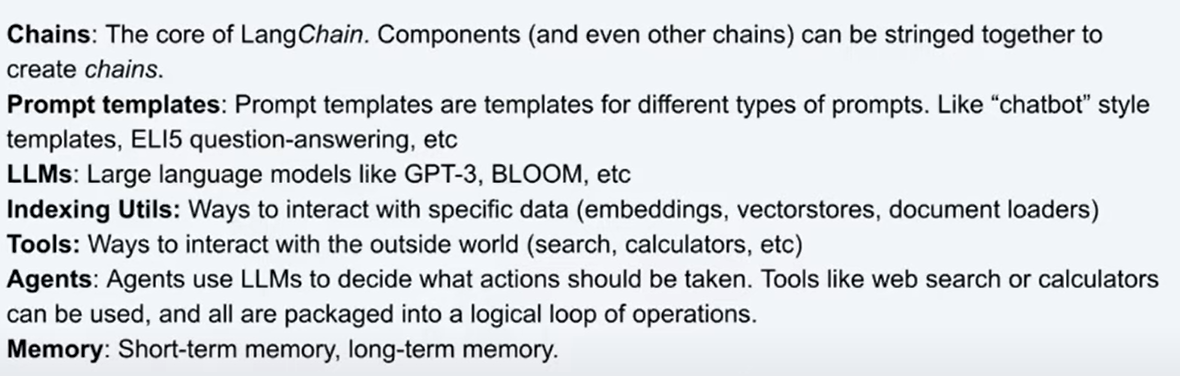
\includegraphics[width=\linewidth,keepaspectratio]{langchain1}
\end{center}	  

{\tiny (Ref: Building the Future with LLMs, LangChain, \& Pinecone)}
\end{frame}


%%%%%%%%%%%%%%%%%%%%%%%%%%%%%%%%%%%%%%%%%%%%%%%%%%%%%%%%%%%%%%%%%%%%%%%%%%%%%%%%%%
\begin{frame}[fragile]\frametitle{LangChain Data Loaders}

There are a lot of document loaders: File Loader, Directory Loader, Notion, ReadTheDocs, HTML, PDF, PowerPoint, Email, GoogleDrive, Obsidian, Roam, EverNote, YouTube, Hacker News, GitBook, S3 File, S3 Directory, GCS File, GCS Directory, Web Base, IMSDb, AZLyrics, College Confidential, Gutenberg, Airbyte Json, CoNLL-U, iFixit, Notebook, Copypaste, CSV, Facebook Chat, Image, Markdown, SRT, Telegram, URL, Word Document, Blackboard

Langchain will chunk the documents and then index its vectors.

\begin{lstlisting}
from langchain.document_loaders import TextLoader
loader = TextLoader('state_of_the_union.txt')
from langchain.indexes import VectorstoreIndexCreator
index = VectorstoreIndexCreator().from_loaders([loader])
query = "What did the president say about Ketanji Brown Jackson"
index.query(query)
\end{lstlisting}	  

\end{frame}

%%%%%%%%%%%%%%%%%%%%%%%%%%%%%%%%%%%%%%%%%%%%%%%%%%%%%%%%%%%%%%%%%%%%%%%%%%%%%%%%%%
\begin{frame}[fragile]\frametitle{LangChain Memory}

Keeps chat history in memory. You can also summarize the chat history.

\begin{lstlisting}
from langchain.llms import OpenAI
from langchain.prompts import PromptTemplate
from langchain.chains import ConversationChain
from langchain.memory import ConversationBufferWindowMemory, CombinedMemory, ConversationSummaryMemory


conv_memory = ConversationBufferWindowMemory(
    memory_key="chat_history_lines",
    input_key="input",
    k=1
)

summary_memory = ConversationSummaryMemory(llm=OpenAI(), input_key="input")
# Combined
memory = CombinedMemory(memories=[conv_memory, summary_memory])
_DEFAULT_TEMPLATE = """The following is a friendly conversation between a human and an AI. The AI is talkative and provides lots of specific details from its context. If the AI does not know the answer to a question, it truthfully says it does not know.

\end{lstlisting}	  

\end{frame}


%%%%%%%%%%%%%%%%%%%%%%%%%%%%%%%%%%%%%%%%%%%%%%%%%%%%%%%%%%%%%%%%%%%%%%%%%%%%%%%%%%
\begin{frame}[fragile]\frametitle{LangChain Memory}


\begin{lstlisting}
Summary of conversation:
{history}
Current conversation:
{chat_history_lines}
Human: {input}
AI:"""
PROMPT = PromptTemplate(
    input_variables=["history", "input", "chat_history_lines"], template=_DEFAULT_TEMPLATE
)
llm = OpenAI(temperature=0)
conversation = ConversationChain(
    llm=llm, 
    verbose=True, 
    memory=memory,
    prompt=PROMPT
)

conversation.run("Hi!")
conversation.run("Can you tell me a joke?")
conversation.run("Can you tell me a similar joke?")
\end{lstlisting}	  

\end{frame}


%%%%%%%%%%%%%%%%%%%%%%%%%%%%%%%%%%%%%%%%%%%%%%%%%%%%%%%%%%%%%%%%%%%%%%%%%%%%%%%%%%
\begin{frame}[fragile]\frametitle{Building Blocks: Inputs}

Input types that LLMs accept

\begin{itemize}
\item Simple string \lstinline|my_text = "What day comes after Friday?"|
\item For the models that handle conversations, chat message type input is needed. There are three message types to label who the sender is: system (Role), human (Prompt), and assistant (AI) for response.
\item Some LLM models accept a document as their input. A document not only includes the page content but also some meta-data such as the source and creation time.
\end{itemize}

{\tiny (Ref: Techy Stuff 3: Notes on LangChain Library - Bill)}

\begin{lstlisting}
chat = ChatOpenAI(temperature=.7, openai_api_key=openai_api_key)

chat([ SystemMessage(content="You are a nice AI bot that helps a user figure out what to eat in one short sentence"),
        HumanMessage(content="I like tomatoes, what should I eat?") ])
Document(page_content="This is my document. It is full of text that I've gathered from other places",
         metadata={'my_document_id' =234234,'my_document_source' = "The LangChain Papers",    'my_document_create_time' = 1680013019 })
\end{lstlisting}	  


\end{frame}

%%%%%%%%%%%%%%%%%%%%%%%%%%%%%%%%%%%%%%%%%%%%%%%%%%%%%%%%%%%%%%%%%%%%%%%%%%%%%%%%%%
\begin{frame}[fragile]\frametitle{Building Blocks: Models}

You provide input of a certain type (text, chat, or document) to a model, and the model will spit out a result for you.

\begin{itemize}
\item To use an LLM, you can import it from LangChain’s LLMS module.
\item The most common model is the language model that accepts a simple string input
\end{itemize}

{\tiny (Ref: Techy Stuff 3: Notes on LangChain Library - Bill)}

\begin{lstlisting}
from langchain.llms import OpenAI
llm = OpenAI(model_name="text-ada-001", openai_api_key=openai_api_key)
llm("What day comes after Friday?")
\end{lstlisting}	  


\end{frame}

%%%%%%%%%%%%%%%%%%%%%%%%%%%%%%%%%%%%%%%%%%%%%%%%%%%%%%%%%%%%%%%%%%%%%%%%%%%%%%%%%%
\begin{frame}[fragile]\frametitle{Building Blocks: Models}

 The chat model allows AI to generate a response from an array of conversations. Each conversation can be initiated by a different party such as the system, a human, and an AI assistant

{\tiny (Ref: Techy Stuff 2: Notes on Prompt Engineering - Bill)}

\begin{lstlisting}
from langchain.chat_models import ChatOpenAI
from langchain.schema import HumanMessage, SystemMessage, AIMessage

chat = ChatOpenAI(temperature=1, openai_api_key=openai_api_key)
chat(
    [
        SystemMessage(content="You are an unhelpful AI bot that makes a joke at whatever the user says"),
        HumanMessage(content="I would like to go to New York, how should I do this?")
    ]
)
\end{lstlisting}	  
\end{frame}


%%%%%%%%%%%%%%%%%%%%%%%%%%%%%%%%%%%%%%%%%%%%%%%%%%%%%%%%%%%%%%%%%%%%%%%%%%%%%%%%%%
\begin{frame}[fragile]\frametitle{Building Blocks: Models}

Text embedding model turns a string of text into a vector representation. A vector is simply an array of numbers of a set length depending on the embedding model. Each number is called a dimension.

{\tiny (Ref: Techy Stuff 2: Notes on Prompt Engineering - Bill)}

\begin{lstlisting}
from langchain.embeddings import OpenAIEmbeddings

embeddings = OpenAIEmbeddings(openai_api_key=openai_api_key)

text = "Hi! It's time for the beach"

text_embedding = embeddings.embed_query(text)
print (f"Your embedding is length {len(text_embedding)}")
print (f"Here's a sample: {text_embedding[:5]}...")

// Here's a sample: [-0.00020583387231454253, -0.003205398330464959, -0.0008301587076857686, -0.01946892775595188, -0.015162716619670391]...
\end{lstlisting}	  
\end{frame}


%%%%%%%%%%%%%%%%%%%%%%%%%%%%%%%%%%%%%%%%%%%%%%%%%%%%%%%%%%%%%%%%%%%%%%%%%%%%%%%%%%
\begin{frame}[fragile]\frametitle{Building Blocks: Prompts}

\begin{itemize}
\item You can pass a static prompt to a model and get a result, but it will be boring. 
\item For a model to provide a relevant output dynamically based on the user and the context, you need a smarter way to construct the prompt.
\item With the prompt template class, you can create a prompt that includes variables, so the content of a template can be super flexible, which can even pull data from external sources.
\end{itemize}

{\tiny (Ref: Techy Stuff 3: Notes on LangChain Library - Bill)}

	  
\end{frame}


%%%%%%%%%%%%%%%%%%%%%%%%%%%%%%%%%%%%%%%%%%%%%%%%%%%%%%%%%%%%%%%%%%%%%%%%%%%%%%%%%%
\begin{frame}[fragile]\frametitle{Building Blocks: Prompts}

\begin{lstlisting}
from langchain.llms import OpenAI
from langchain import PromptTemplate

llm = OpenAI(model_name="text-davinci-003", openai_api_key=openai_api_key)

# Notice "location" below, that is a placeholder for another value later
template = """
I really want to travel to {location}. What should I do there?

Respond in one short sentence
"""

prompt = PromptTemplate(input_variables=["location"],template=template)
final_prompt = prompt.format(location='Rome')
\end{lstlisting}	  
\end{frame}

%%%%%%%%%%%%%%%%%%%%%%%%%%%%%%%%%%%%%%%%%%%%%%%%%%%%%%%%%%%%%%%%%%%%%%%%%%%%%%%%%%
\begin{frame}[fragile]\frametitle{Building Blocks: Example Selector}

\begin{itemize}
\item One common practice to enrich a prompt is through few-shot prompting, you append a few examples before a user’s actual question/input to teach the machine how it should approach a question and format its answer.
\item If you put all the examples you have into a prompt, the length of the input might exceed the max tokens, and the API cost will be exorbitantly high.
\item Example Selector can automatically pick the relevant examples that closely relate to the user’s input and append them to a prompt for you.
\end{itemize}

{\tiny (Ref: Techy Stuff 3: Notes on LangChain Library - Bill)}

\end{frame}

%%%%%%%%%%%%%%%%%%%%%%%%%%%%%%%%%%%%%%%%%%%%%%%%%%%%%%%%%%%%%%%%%%%%%%%%%%%%%%%%%%
\begin{frame}[fragile]\frametitle{Building Blocks: Example Selector}

\begin{lstlisting}
from langchain.prompts import FewShotPromptTemplate, PromptTemplate
from langchain.llms import OpenAI

llm = OpenAI(model_name="text-davinci-003", openai_api_key=openai_api_key)

example_prompt = PromptTemplate(
    input_variables=["input", "output"],
    template="Example Input: {input}\nExample Output: {output}",
)

# Examples of locations that nouns are found
examples = [
    {"input": "pirate", "output": "ship"},
    {"input": "pilot", "output": "plane"},
    {"input": "driver", "output": "car"},
    {"input": "tree", "output": "ground"},
    {"input": "bird", "output": "nest"},
]
\end{lstlisting}	  
\end{frame}

%%%%%%%%%%%%%%%%%%%%%%%%%%%%%%%%%%%%%%%%%%%%%%%%%%%%%%%%%%%%%%%%%%%%%%%%%%%%%%%%%%
\begin{frame}[fragile]\frametitle{Building Blocks: Example Selector}

\begin{lstlisting}
# SemanticSimilarityExampleSelector will select examples that are similar to your input by semantic meaning

example_selector = SemanticSimilarityExampleSelector.from_examples(
    # This is the list of examples available to select from.
    examples, 
    
    # This is the embedding class used to produce embeddings which are used to measure semantic similarity.
    OpenAIEmbeddings(openai_api_key=openai_api_key), 
    
    # This is the VectorStore class that is used to store the embeddings and do a similarity search over.
    FAISS, 
    
    # This is the number of examples to produce.
    k=2
)

similar_prompt = FewShotPromptTemplate(
    # The object that will help select examples
    example_selector=example_selector,
    
    # Your prompt
    example_prompt=example_prompt,
    
    # Customizations that will be added to the top and bottom of your prompt
    prefix="Give the location an item is usually found in",
    suffix="Input: {noun}\nOutput:",
    
    # What inputs your prompt will receive
    input_variables=["noun"],
)

llm(similar_prompt.format(noun=my_noun))
\end{lstlisting}	  
\end{frame}

%%%%%%%%%%%%%%%%%%%%%%%%%%%%%%%%%%%%%%%%%%%%%%%%%%%%%%%%%%%%%%%%%%%%%%%%%%%%%%%%%%
\begin{frame}[fragile]\frametitle{Building Blocks: Indexes}

\begin{itemize}
\item What should you do if you want to ask GPT to summarize a 300-page novel for you? 
\item GPT has set a max token on the user’s input so you cannot just copy and paste the whole document into a prompt. 
\item For a model to consume a longer text, we have to use a technique called indexes, and here are the steps we have to perform:
\begin{itemize}
\item Load the document (think of it as a 300-page novel in PDF format)
\item Split the text into chunks (set the max tokens for each chunk)
\item Embed the chunks into vectors with the embedding model
\item Store them in a vector database
\item Retrieve the relevant chunks when building a prompt dynamically
\end{itemize}
\end{itemize}

{\tiny (Ref: Techy Stuff 3: Notes on LangChain Library - Bill)}

\end{frame}

%%%%%%%%%%%%%%%%%%%%%%%%%%%%%%%%%%%%%%%%%%%%%%%%%%%%%%%%%%%%%%%%%%%%%%%%%%%%%%%%%%
\begin{frame}[fragile]\frametitle{Building Blocks: Indexes}

Here is the example code:


\begin{lstlisting}
from langchain.document_loaders import TextLoader
from langchain.text_splitter import RecursiveCharacterTextSplitter
from langchain.vectorstores import FAISS
from langchain.embeddings import OpenAIEmbeddings

loader = TextLoader('data/PaulGrahamEssays/worked.txt')
documents = loader.load()
text_splitter = RecursiveCharacterTextSplitter(chunk_size=1000, chunk_overlap=50)
texts = text_splitter.split_documents(documents)
embeddings = OpenAIEmbeddings(openai_api_key=openai_api_key)
db = FAISS.from_documents(texts, embeddings)
retriever = db.as_retriever()
docs = retriever.get_relevant_documents("what types of things did the author want to build?")
\end{lstlisting}	  
\end{frame}


%%%%%%%%%%%%%%%%%%%%%%%%%%%%%%%%%%%%%%%%%%%%%%%%%%%%%%%%%%%%%%%%%%%%%%%%%%%%%%%%%%
\begin{frame}\frametitle{Chains}

\begin{itemize}
\item Enable users to combine multiple components together to create a single, coherent application.
\item Example: takes user input, formats it using a PromptTemplate, and then passes the formatted response to a Large Language Model (LLM) for processing.
\item Sequential chains: output of the first LLM becomes the input to the second LLM and so on
\end{itemize}

\begin{center}
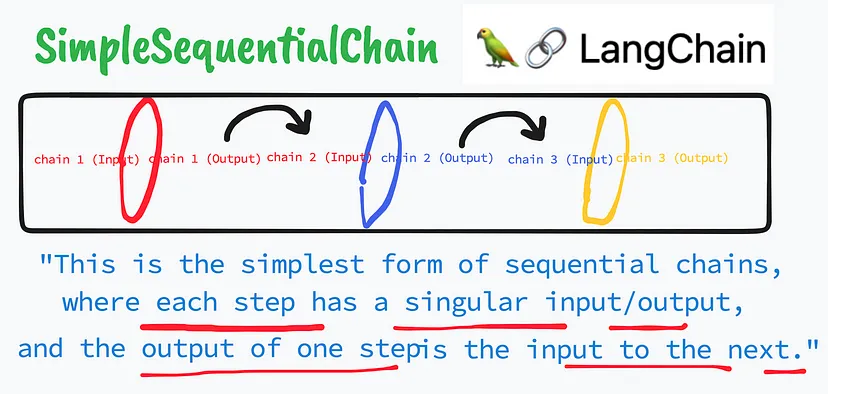
\includegraphics[width=0.8\linewidth,keepaspectratio]{langchain5}
\end{center}	  


{\tiny (Ref: Getting started with LangChain - Avra)}
\end{frame}

%%%%%%%%%%%%%%%%%%%%%%%%%%%%%%%%%%%%%%%%%%%%%%%%%%%%%%%%%%%%%%%%%%%%%%%%%%%%%%%%%%
\begin{frame}[fragile]\frametitle{Chains: Combining LLMs with other components}

Combining LLMs with other components to create an application. Some examples are:


\begin{itemize}
\item Combining LLMs with prompt templates 
\item Combining multiple LLMs sequentially by taking the first LLM’s output as the input for the second LLM 
\item Combining LLMs with external data, e.g., for question answering 
\item Combining LLMs with long-term memory, e.g., for chat history
\end{itemize}

{\tiny (Ref: Getting Started with LangChain: A Beginner’s Guide to Building LLM-Powered Applications by Leonie Monigatti)}

\end{frame}

%%%%%%%%%%%%%%%%%%%%%%%%%%%%%%%%%%%%%%%%%%%%%%%%%%%%%%%%%%%%%%%%%%%%%%%%%%%%%%%%%%
\begin{frame}[fragile]\frametitle{Combining LLMs with prompt templates}



\begin{lstlisting}
from langchain.chains import LLMChain

chain = LLMChain(llm = llm, 
                  prompt = prompt)

# Run the chain only specifying the input variable.
chain.run("colorful socks")
\end{lstlisting}


\end{frame}

%%%%%%%%%%%%%%%%%%%%%%%%%%%%%%%%%%%%%%%%%%%%%%%%%%%%%%%%%%%%%%%%%%%%%%%%%%%%%%%%%%
\begin{frame}[fragile]\frametitle{Combining multiple LLMs sequentially}

If we want to use the output of this first LLM as the input for a second LLM, we can use a SimpleSequentialChain:

\begin{lstlisting}
from langchain.chains import LLMChain, SimpleSequentialChain

# Define the first chain as in the previous code example
# ...

# Create a second chain with a prompt template and an LLM
second_prompt = PromptTemplate(
    input_variables=["company_name"],
    template="Write a catchphrase for the following company: {company_name}",
)

chain_two = LLMChain(llm=llm, prompt=second_prompt)

# Combine the first and the second chain 
overall_chain = SimpleSequentialChain(chains=[chain, chain_two], verbose=True)

# Run the chain specifying only the input variable for the first chain.
catchphrase = overall_chain.run("colorful socks")
\end{lstlisting}


\end{frame}

%%%%%%%%%%%%%%%%%%%%%%%%%%%%%%%%%%%%%%%%%%%%%%%%%%%%%%%%%%%%%%%%%%%%%%%%%%%%%%%%%%
\begin{frame}[fragile]\frametitle{Combining LLMs with external data, e.g., for question answering}

\begin{itemize}
\item Load the external data with a document loader from PDFs and emails to websites and YouTube videos. 
\item Now that you have your external data ready to go as documents , you can index it with a text embedding model  in a vector database, a VectorStore.  
\item Now you can do a variety of things with this external data. 
\item Let’s use it for a question-answering task with an information retriever
\end{itemize}



\end{frame}

%%%%%%%%%%%%%%%%%%%%%%%%%%%%%%%%%%%%%%%%%%%%%%%%%%%%%%%%%%%%%%%%%%%%%%%%%%%%%%%%%%
\begin{frame}[fragile]\frametitle{Combining LLMs with external data, e.g., for question answering}


\begin{lstlisting}
# pip install youtube-transcript-api
# pip install pytube

from langchain.document_loaders import YoutubeLoader
loader = YoutubeLoader.from_youtube_url("https://www.youtube.com/watch?v=dQw4w9WgXcQ")
documents = loader.load()

from langchain.vectorstores import FAISS
db = FAISS.from_documents(documents, embeddings)

from langchain.chains import RetrievalQA
retriever = db.as_retriever()

qa = RetrievalQA.from_chain_type(
    llm=llm, 
    chain_type="stuff", 
    retriever=retriever, 
    return_source_documents=True)

query = "What am I never going to do?"
result = qa({"query": query})

print(result['result'])
\end{lstlisting}


\end{frame}


%%%%%%%%%%%%%%%%%%%%%%%%%%%%%%%%%%%%%%%%%%%%%%%%%%%%%%%%%%%%%%%%%%%%%%%%%%%%%%%%%%
\begin{frame}[fragile]\frametitle{Combining LLMs with long-term memory}

Remembering previous conversations. LangChain solves this problem by providing several different options for dealing with chat history :

\begin{itemize}
\item keep all conversations,
\item keep the latest k conversations,
\item summarize the conversation.
\end{itemize}

\begin{lstlisting}
from langchain import ConversationChain

conversation = ConversationChain(llm=llm, verbose=True)

conversation.predict(input="Alice has a parrot.")

conversation.predict(input="Bob has two cats.")

conversation.predict(input="How many pets do Alice and Bob have?")
\end{lstlisting}


\end{frame}


%%%%%%%%%%%%%%%%%%%%%%%%%%%%%%%%%%%%%%%%%%%%%%%%%%%%%%%%%%%%%%%%%%%%%%%%%%%%%%%%%%
\begin{frame}[fragile]\frametitle{LangChain Chain}


\begin{lstlisting}
from langchain.chat_models import ChatOpenAI
from langchain import LLMChain
from langchain.prompts.chat import (
    ChatPromptTemplate,
    HumanMessagePromptTemplate,
)
human_message_prompt = HumanMessagePromptTemplate(
        prompt=PromptTemplate(
            template="What is a good name for a company that makes {product}?",
            input_variables=["product"],
        )
    )
chat_prompt_template = ChatPromptTemplate.from_messages([human_message_prompt])
chat = ChatOpenAI(temperature=0.9)
chain = LLMChain(llm=chat, prompt=chat_prompt_template)
print(chain.run("colorful socks"))

\end{lstlisting}	  

\end{frame}


%%%%%%%%%%%%%%%%%%%%%%%%%%%%%%%%%%%%%%%%%%%%%%%%%%%%%%%%%%%%%%%%%%%%%%%%%%%%%%%%%%
\begin{frame}[fragile]\frametitle{LangChain Chain}


\begin{lstlisting}

second_prompt = PromptTemplate(
    input_variables=["company_name"],
    template="Write a catchphrase for the following company: {company_name}",
)
chain_two = LLMChain(llm=llm, prompt=second_prompt)

from langchain.chains import SimpleSequentialChain
overall_chain = SimpleSequentialChain(chains=[chain, chain_two], verbose=True)

# Run the chain specifying only the input variable for the first chain.
catchphrase = overall_chain.run("colorful socks")
print(catchphrase)
\end{lstlisting}	  

\end{frame}


%%%%%%%%%%%%%%%%%%%%%%%%%%%%%%%%%%%%%%%%%%%%%%%%%%%%%%%%%%%%%%%%%%%%%%%%%%%%%%%%%%
\begin{frame}[fragile]\frametitle{Agents: Accessing other tools}


\begin{itemize}
\item Despite being quite powerful, LLMs have some limitations: they lack contextual information (e.g., access to specific knowledge not contained in training data), they can become outdated quickly (e.g., GPT-4 was trained on data before September 2021), and they are bad at math.
\item we need to give them access to supplementary tools such as search (e.g., Google Search), calculators (e.g., Python REPL or Wolfram Alpha), and lookups (e.g., Wikipedia).
\item Additionally, we need agents that make decisions about which tools to use to accomplish a task based on the LLM’s output.
\end{itemize}

\begin{lstlisting}
# pip install wikipedia
from langchain.agents import load_tools
from langchain.agents import initialize_agent
from langchain.agents import AgentType

tools = load_tools(["wikipedia", "llm-math"], llm=llm)
agent = initialize_agent(tools, llm, agent=AgentType.ZERO_SHOT_REACT_DESCRIPTION, 
                         verbose=True)

agent.run("When was Barack Obama born? How old was he in 2022?")
\end{lstlisting}


\end{frame}


%%%%%%%%%%%%%%%%%%%%%%%%%%%%%%%%%%%%%%%%%%%%%%%%%%%%%%%%%%%%%%%%%%%%%%%%%%%%%%%%%%
\begin{frame}[fragile]\frametitle{LangChain Agent}

Use various LLMs with external tools, like 'serpapi' to do Google search.

First search api finds who the girlfreind is, then it uses calculator to do the maths.

\begin{lstlisting}
from langchain.agents import load_tools
from langchain.agents import initialize_agent

tools = load_tools(["serpapi", "llm-math"], llm=gpt3)
agent = initialize_agent(tools, llm=gpt3, agent="zero-shot-react-description", verbose=True)
agent.run("Who is Leo DiCaprio's girlfriend? What is her current age raised to the 0.43 power?")
\end{lstlisting}	  

\end{frame}

%%%%%%%%%%%%%%%%%%%%%%%%%%%%%%%%%%%%%%%%%%%%%%%%%%%%%%%%%%%%%%%%%%%%%%%%%%%%%%%%%%
\begin{frame}[fragile]\frametitle{Chains, another example}

{\tiny (Ref: Getting started with LangChain - Avra)}


\begin{lstlisting}
    # Chain 1: Generating a rephrased version of the user's question
    template = """{question}\n\n"""
    prompt_template = PromptTemplate(input_variables=["question"], template=template)
    question_chain = LLMChain(llm=llm, prompt=prompt_template)

    # Chain 2: Generating assumptions made in the statement
    template = """Here is a statement:
        {statement}
        Make a bullet point list of the assumptions you made when producing the above statement.\n\n"""
    prompt_template = PromptTemplate(input_variables=["statement"], template=template)
    assumptions_chain = LLMChain(llm=llm, prompt=prompt_template)
    assumptions_chain_seq = SimpleSequentialChain(
        chains=[question_chain, assumptions_chain], verbose=True
    )

\end{lstlisting}

\end{frame}

%%%%%%%%%%%%%%%%%%%%%%%%%%%%%%%%%%%%%%%%%%%%%%%%%%%%%%%%%%%%%%%%%%%%%%%%%%%%%%%%%%
\begin{frame}[fragile]\frametitle{Chains}

{\tiny (Ref: Getting started with LangChain - Avra)}


\begin{lstlisting}
    # Chain 3: Fact checking the assumptions
    template = """Here is a bullet point list of assertions:
    {assertions}
    For each assertion, determine whether it is true or false. If it is false, explain why.\n\n"""
    prompt_template = PromptTemplate(input_variables=["assertions"], template=template)
    fact_checker_chain = LLMChain(llm=llm, prompt=prompt_template)
    fact_checker_chain_seq = SimpleSequentialChain(
        chains=[question_chain, assumptions_chain, fact_checker_chain], verbose=True)
    # Final Chain: Generating the final answer to the user's question based on the facts and assumptions
    template = """In light of the above facts, how would you answer the question '{}'""".format(user_question)
    template = """{facts}\n""" + template
    prompt_template = PromptTemplate(input_variables=["facts"], template=template)
    answer_chain = LLMChain(llm=llm, prompt=prompt_template)
    overall_chain = SimpleSequentialChain(
        chains=[question_chain, assumptions_chain, fact_checker_chain, answer_chain],
        verbose=True,)
\end{lstlisting}


\end{frame}

%%%%%%%%%%%%%%%%%%%%%%%%%%%%%%%%%%%%%%%%%%%%%%%%%%%%%%%%%%%%%%%%%%%%%%%%%%%%%%%%%%
\begin{frame}\frametitle{Chains}

The SimpleSequentialChain combines several chains of operations to run a pipeline. 

\begin{itemize}
\item question\_chain: This chain takes the user's question as input and returns it as output. 
\item assumptions\_chain: This chain takes the output from question\_chain as input and produces a bullet-point list of assumptions based on a statement related to the question. 
\item fact\_checker\_chain: This chain takes the outputs from question\_chain and assumptions\_chain as inputs and produces a bullet-point list of assertions based on the question and assumptions.
\item answer\_chain: This chain takes the outputs from question\_chain, assumptions\_chain, and fact\_checker\_chain as inputs and produces an answer to the user's question based on the facts generated by the previous chains.
\end{itemize}


{\tiny (Ref: Getting started with LangChain - Avra)}
\end{frame}


%%%%%%%%%%%%%%%%%%%%%%%%%%%%%%%%%%%%%%%%%%%%%%%%%%%%%%%%%%%%%%%%%%%%%%%%%%%%%%%%%%
\begin{frame}\frametitle{Prompt Engineering}

\begin{center}
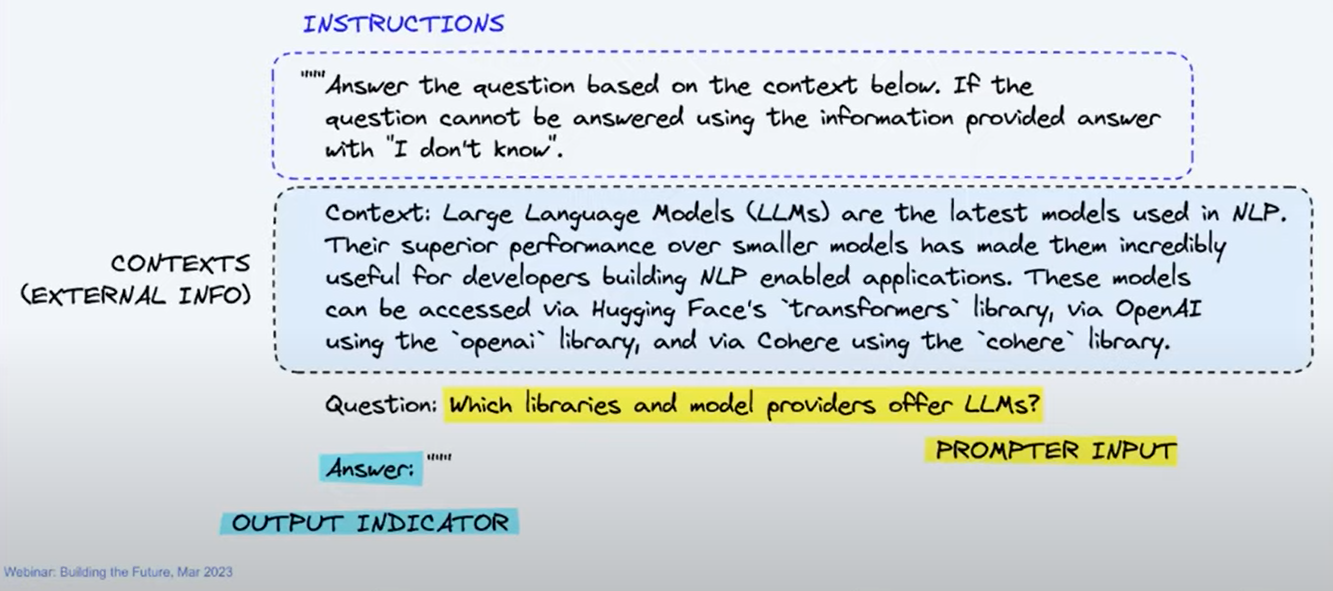
\includegraphics[width=\linewidth,keepaspectratio]{langchain2}
\end{center}	  

{\tiny (Ref: Building the Future with LLMs, LangChain, \& Pinecone)}
\end{frame}
